\documentclass[10pt]{beamer}
\usepackage[utf8]{inputenc}
\usepackage{tikz}
\usetikzlibrary{shapes, arrows.meta, positioning}

\usepackage[absolute,overlay]{textpos}
\usepackage{graphicx}
\usepackage{listings}
\lstset{
  language=Python,
  basicstyle=\ttfamily\scriptsize,
  commentstyle=\color{gray},
  keywordstyle=\color{blue},
  stringstyle=\color{red},
  showstringspaces=false,
  numbers=left,
  numberstyle=\tiny,
  frame=single,
  breaklines=true,
}

\mode<presentation> {
\usetheme{boxes} % When headline is wanted use Dresden theme instead
\usecolortheme{seagull}
\logo{
\includegraphics[height=1.5cm]{ku_logo_dk}}
\setbeamertemplate{footline}[frame number]
% \setbeamertemplate{footline}{
%   \hspace{1em}
%   \hfill
%   \insertframenumber/\inserttotalframenumber
%   \vspace{1em}
%   \hspace{1em}
%   
\includegraphics[height=2cm]{ku_logo_dk}
%   \hspace{1em}
% }
\setbeamertemplate{navigation symbols}{}
\setbeamertemplate{itemize items}[square]
}


%----------------------------------------------------------------------------------------
%	TITLE PAGE
%----------------------------------------------------------------------------------------

\title[Kickstart-kursus] % bottom of every slide
  {Kickstart Brainstorming\\ 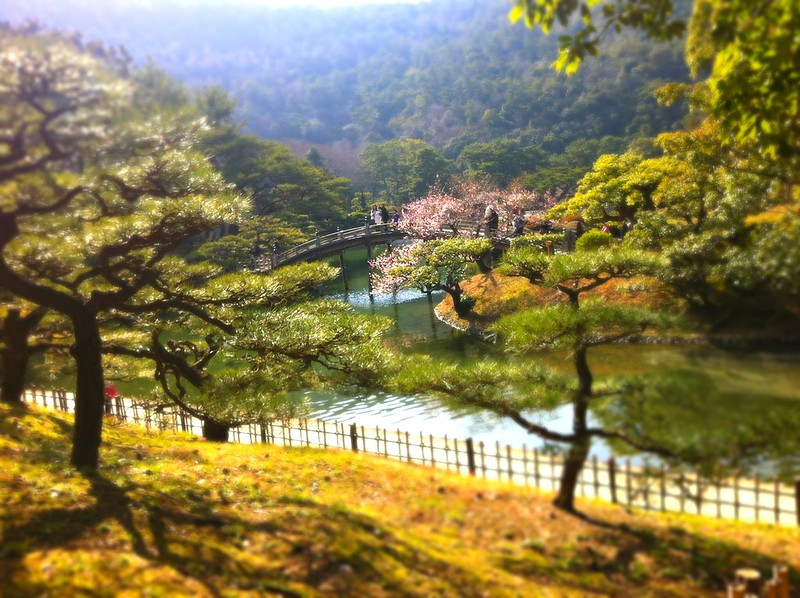
\includegraphics[height=5cm]{images/landscape}} % title page



\author{\footnotesize{Daniel Spikol} \\
          \footnotesize{\texttt{ds@di.ku.dk}}}

\institute {DIKU - Københavns Universitet}

\date[23.august 2023]{23.august 2023}

\begin{document}
\begin{frame}[plain]
\titlepage
\end{frame}

%%----------------------------------------------%%

\begin{frame}{Design IFOs}
  \begin{itemize}
  \item Explore Divergent Thinking
   \item Practice some Brainstorming Techniques
  \item Generate some ideas for a mini project
  \end{itemize}
\end{frame}

%%----------------------------------------------%%
	
\begin{frame}{Modes of Thinking}
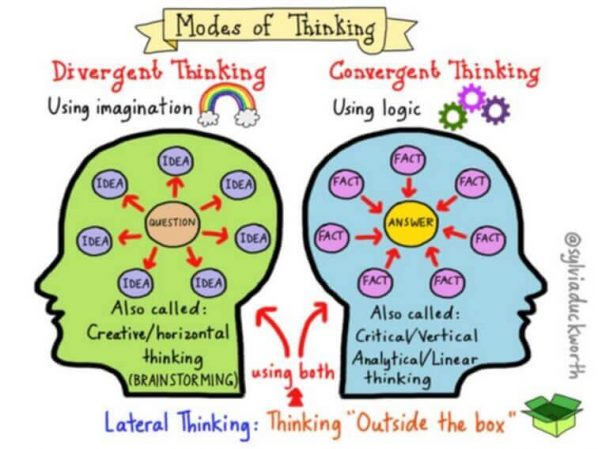
\includegraphics[height=7cm]{images/modes}
\end{frame}

%%----------------------------------------------%%

\begin{frame}{Brainstorming}{General Rules of Engagement}
  \begin{enumerate}
  \item \textbf{Defer judgment} – separating idea generation from idea selection strengthens both activities. 
  \item \textbf{For now, suspend critique} – Know that you’ll have plenty of time to evaluate the ideas after brainstorming. 
  \item \textbf{Encourage wild ideas} – breakout ideas are right next to the absurd ones 
  \item \textbf{Build on the ideas of others} – listen and add to the flow if ideas. This will springboard your group to places no individual can get to on their own 
  \item \textbf{Go for volume} – best way to have a good idea is to have lots of ideas 
  \item \textbf{One conversation at a time} – maintain momentum as a group. Save the side conversations for later. 
  \item \textbf{Headline} – capture the essence quickly and move on. Don’t stall the group by going into a long-winded idea. 
    \end{enumerate}
\end{frame}

%%----------------------------------------------%%

\begin{frame}{Brainstorming}{Techniques for Computer Game Idea}
  \begin{enumerate}
  	\item Begin with a central idea and branch out.
	\item Connect related concepts visually.
	\item Great for exploring components of the game world and mechanics.
    \end{enumerate}
\end{frame}

%%----------------------------------------------%%

\begin{frame}{Brainstorming}{Serious Mindmap}
\begin{center}
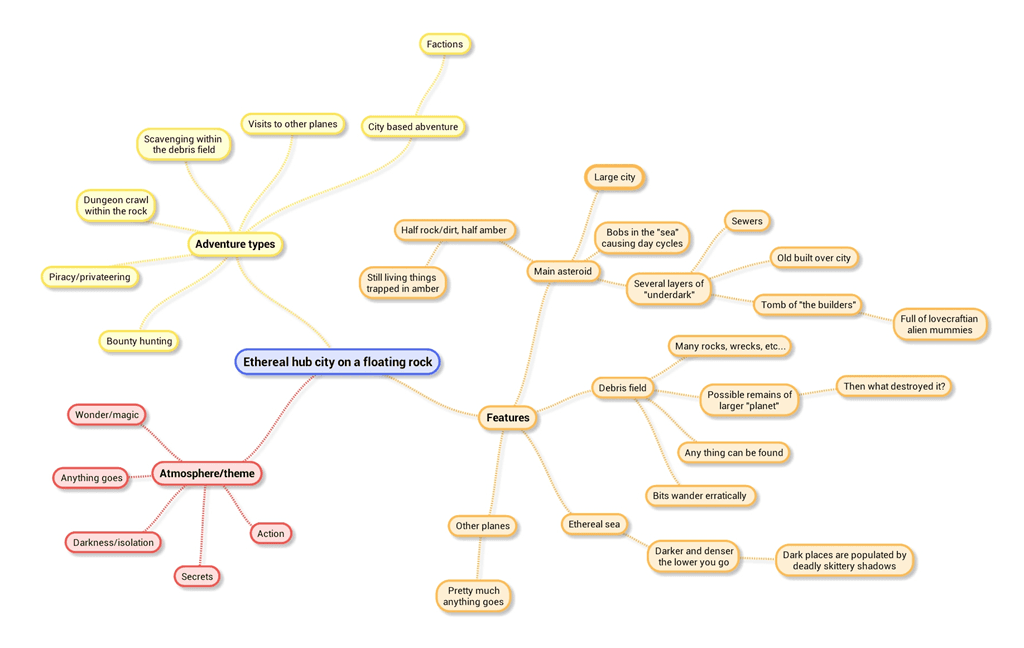
\includegraphics[height=6cm]{images/mindmap}
\end{center}
\end{frame}

%%----------------------------------------------%%

\begin{frame}{Brainstorming}{Sketch like}
\begin{center}
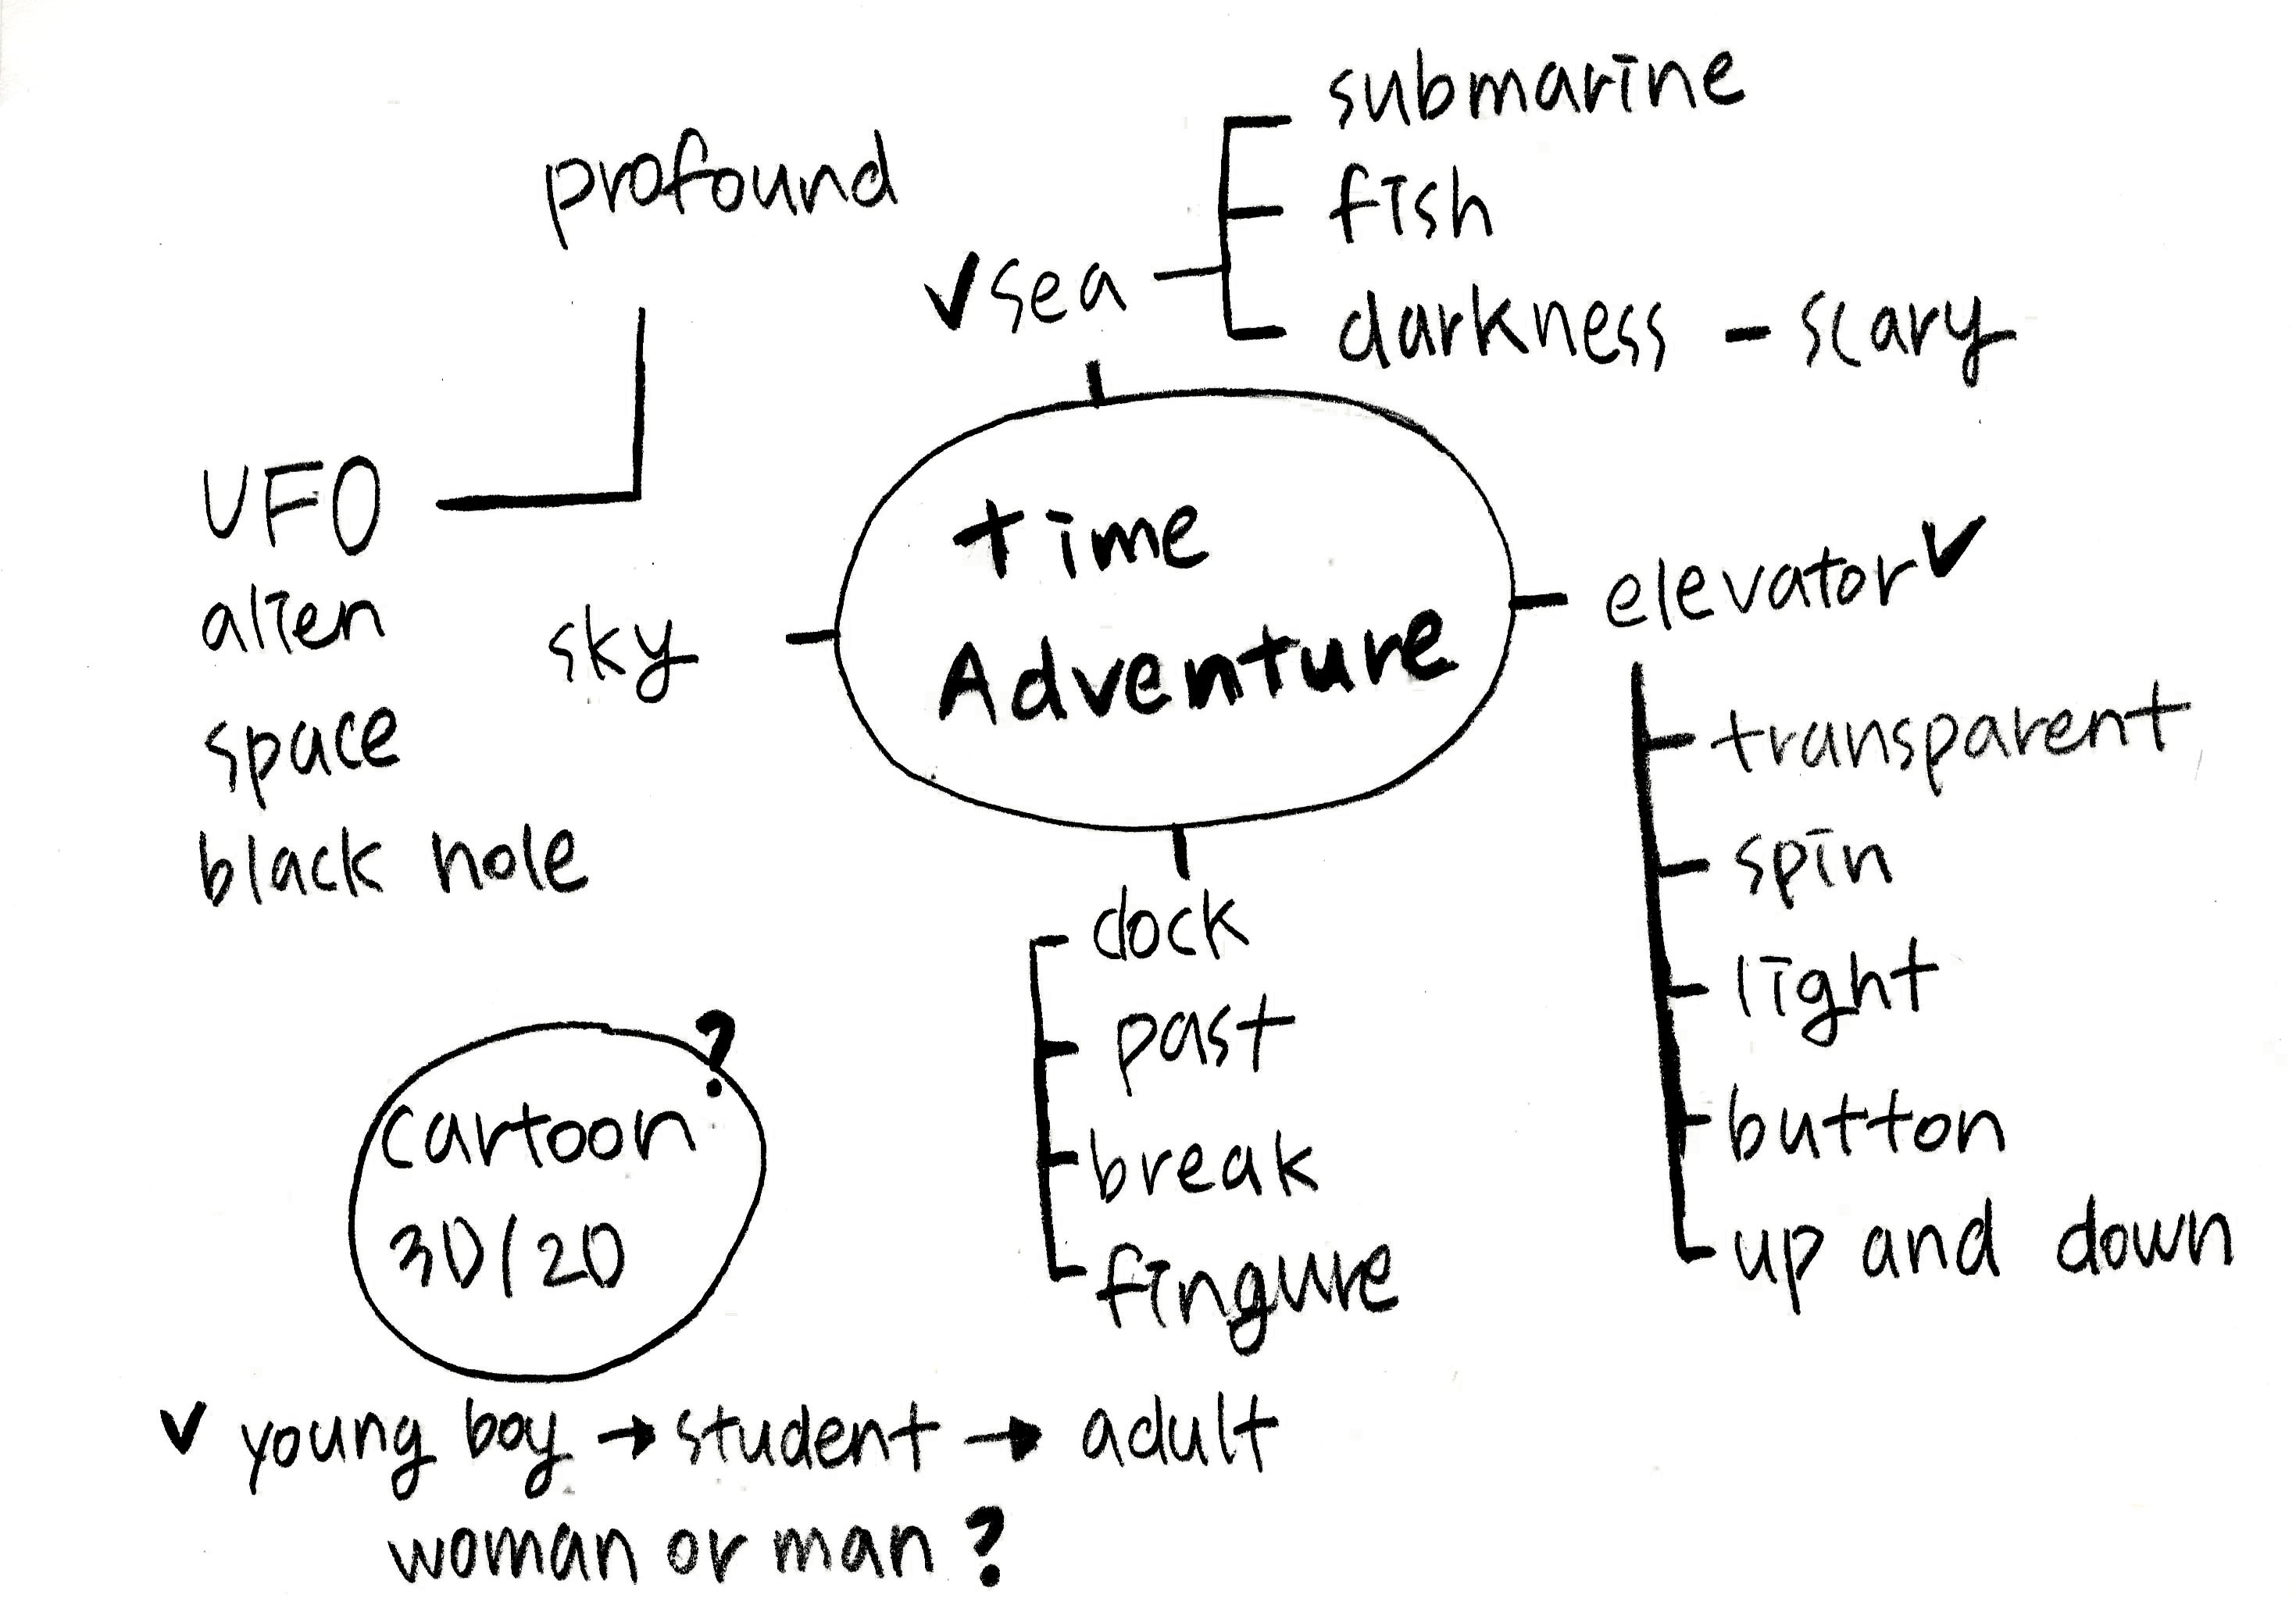
\includegraphics[height=7cm]{images/mindmap2}
\end{center}
\end{frame}

%%----------------------------------------------%%


\begin{frame}{SCAMPER}
\begin{itemize}
\item \textbf{Substitute:} Replace elements of existing games to create something new.
\item \textbf{Combine:} Mix two game concepts or genres.
\item \textbf{Adapt:} Modify an existing game mechanic for a fresh take.
\item \textbf{Modify:} Change the scale, size, or scope of game elements.
\item \textbf{Put to another use:} Repurpose a game mechanic in a novel way.
\item \textbf{Eliminate:} Remove elements to simplify or create a new challenge.
\item \textbf{Reverse:} Flip game dynamics, like making the villain the hero.
\end{itemize}
\end{frame}

%%----------------------------------------------%%

\begin{frame}{Scamper}{Diagram}
\begin{center}
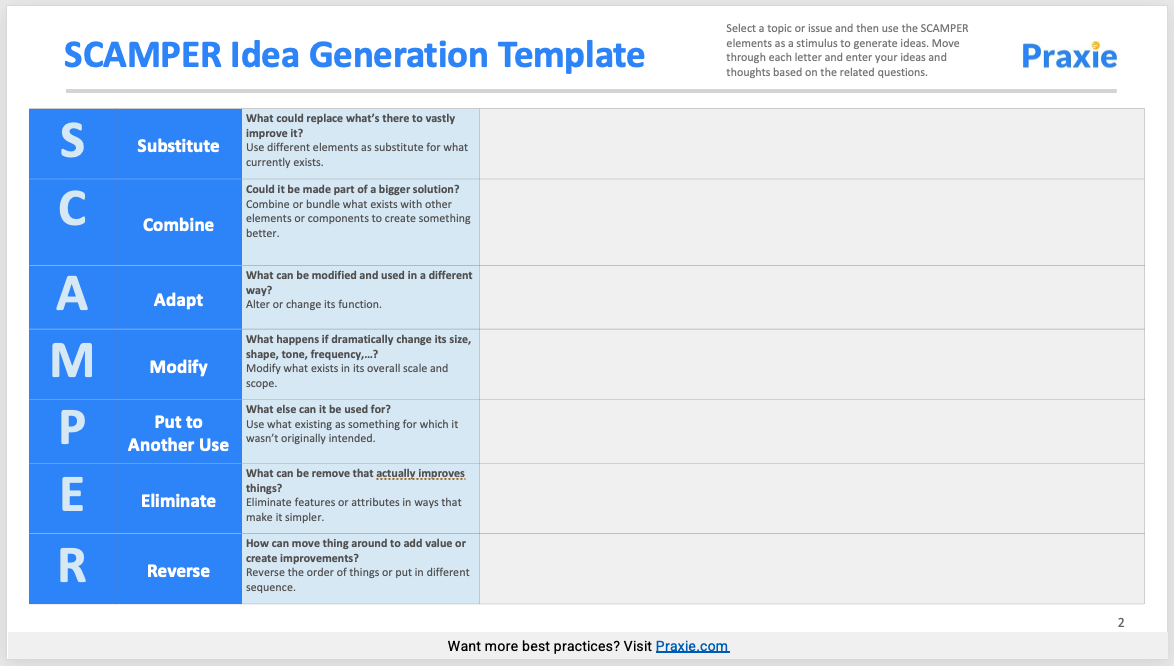
\includegraphics[height=6cm]{images/scamper}
\end{center}
\end{frame}

%%----------------------------------------------%%

\begin{frame}{The ``What If" Technique}
Pose hypothetical situations or challenges.
Example Questions:
\begin{itemize}
\item What if the character couldn't jump?
\item What if the game environment constantly changed?
\item What if there's no antagonist but the environment itself?
\end{itemize}
\end{frame}

%%----------------------------------------------%%

\begin{frame}{Role Play \& Storyboarding}
\begin{center}
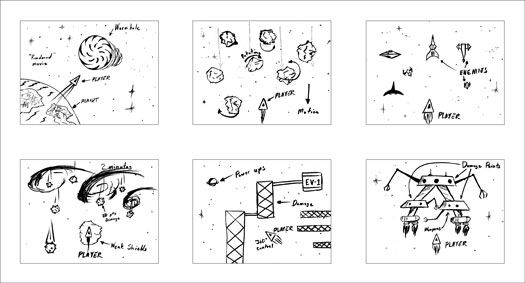
\includegraphics[height=5cm]{images/gamesketch}
\end{center}
\begin{itemize}
\item Role Play: Step into your character's shoes. Act out potential game scenarios.
\item Storyboarding: Visually plot out game scenes, levels, or interactions.
\item These methods help to visualise player experience and narrative flow.
\end{itemize}
\end{frame}

%%----------------------------------------------%%
\begin{frame}{Make it S.U.C.K.}
\begin{center}
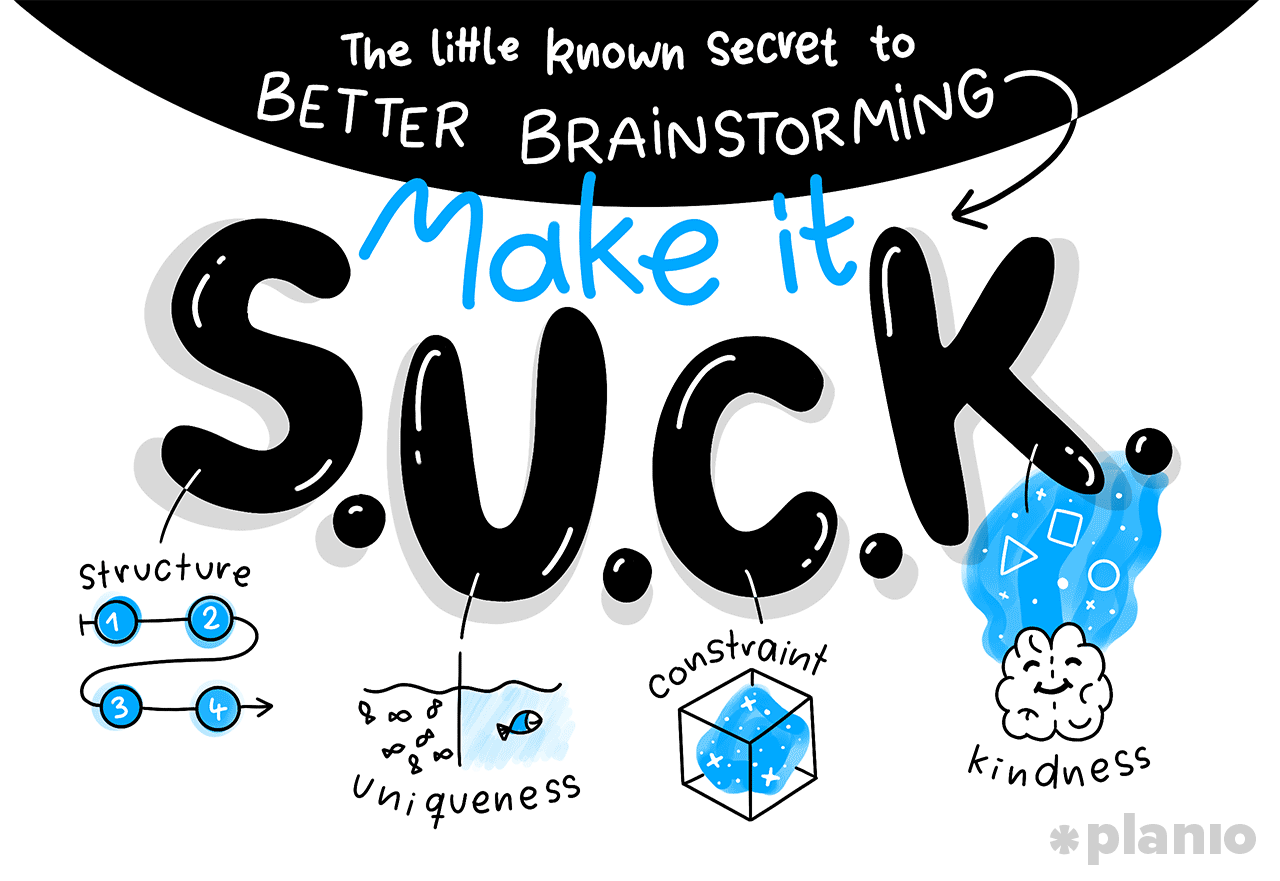
\includegraphics[height=7cm]{images/suck}
\end{center}

\end{frame}

%%----------------------------------------------%%

\begin{frame}{Your Mission}
   	\begin{itemize}
	\item Generate some ideas
	\item Make a team with some people (good idea)
	\item Generate some ideas
	\item Get feedback \& input from everyone
	\end{itemize}
	\begin{center}
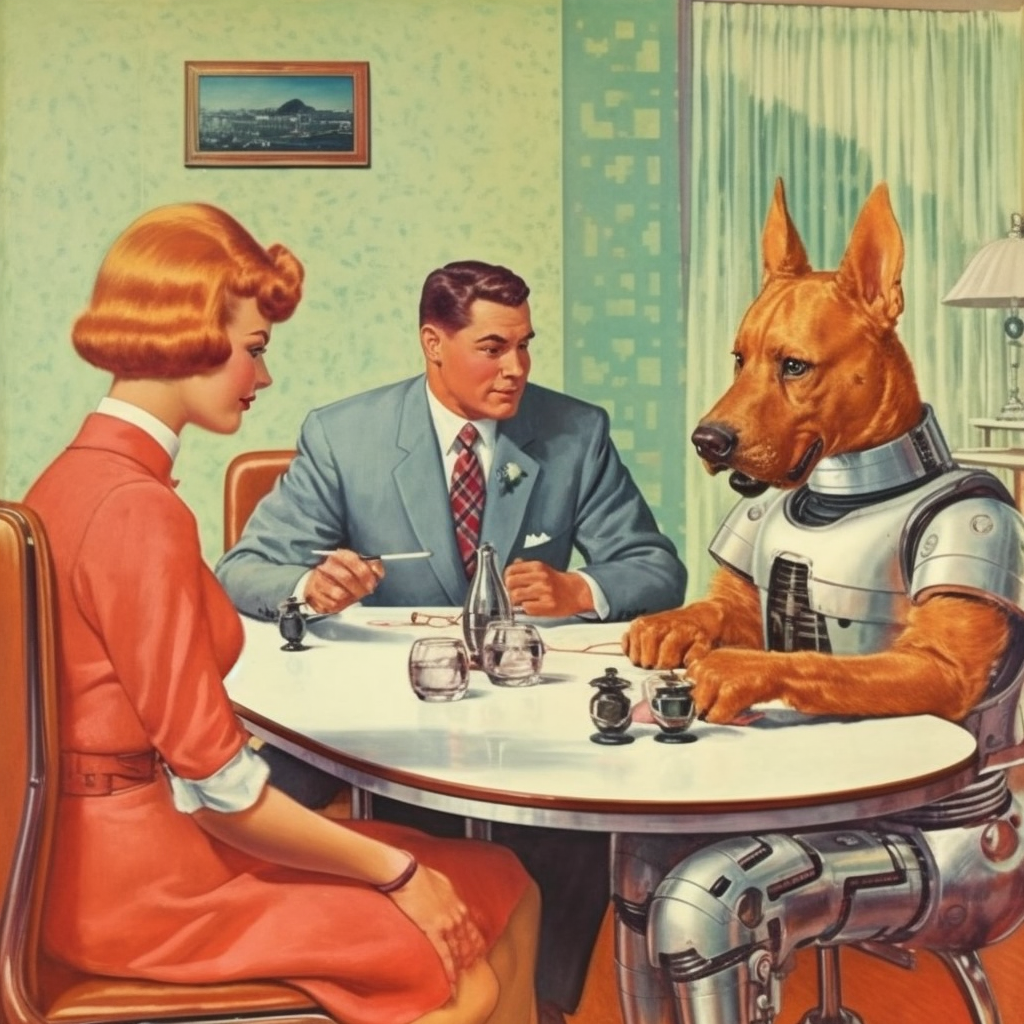
\includegraphics[height=5cm]{images/dog}
\end{center}
\end{frame}
%%----------------------------------------------%%
%%----------------------------------------------%%
%%----------------------------------------------%%
\end{document}